\section{Die Algorithmen auf diesem Markt}
Der Vergleich der RL-Algorithmen findet auf dem in \ref{section:markov} definierten Markt statt.
Dieser Markt wird auf der Testplattform simuliert, die im Rahmen des Bachelorprojektes entwickelt wurde.
Er wird über die Gym-Schnittstelle durch die Agenten angesprochen.
Für die zu vergleichenden Algorithmen werden hauptsächlich die Implementierungen der Bibliothek \textit{Stable Baselines} verwendet. \cite{stable-baselines}
Stable Baselines ist ist eine weit verbreitete eine Open-Source RL-Bibliothek, die in Python geschrieben ist.
Sie baut auf PyTorch auf, einem der beliebtesten Deep-Learning-Frameworks, das in der Forschung weite Verbreitung findet. \cite{NEURIPS2019_9015}
Die in Stable Baselines implementierten Algorithmen entsprechen in den meisten Fällen unmittelbar den vorgeschlagenen Algorithmen der Originalpaper und zeichnen sich durch eine hohe Lesbarkeit des Codes aus.
Alle Hyperparameter sind konfigurierbar.

In dieser Untersuchung der Algorithmen wird stets von den Hyperparametern der Originalpaper ausgegangen.
Weil kaum theoretische Erkenntnisse über die Ermittlung optimaler Hyperparameter vorliegen und diese stets problemspezifisch sind, ist eine erschöpfende Optimierung der Hyperparameter nur mit erheblichem experimentellem Aufwand möglich.
Dazu müssten sehr viele Kombinationen mit jeweils mehreren Läufen durchgeführt werden, was einen nicht zu leistenden Ressourcenaufwand darstellt.
Dennoch wurden an einigen Stellen bessere Hyperparameter gefunden und Aussagen über die Algorithmen über mehrere Hyperparameterkombinationen abgesichert.

Alle Verfahren werden mit neuronalen Netzen durchgeführt, die zwei versteckte Schichten mit je 64 Neuronen haben.
Das Verhalten der Algorithmen für unterschiedliche Netzgrößen ist aber sehr ähnlich, wie die Experimente mit unterschiedlichen Netzgrößen im Bereich [noch zu erstellen] des Anhangs zeigen.
Für den Vergleich der Algorithmen werden diese zunächst innerhalb ihrer Gruppen betrachtet und auf generelle Eignung für dieses Setup geprüft.
Danach werden die Algorithmen, die sich als grundsätzlich geeignet erwiesen haben, hinsichtlich verschiedener Kriterien verglichen.

\section{Q-Learning -- DDPG und TD3}
Bei der Diskussion der Q-Learning-Verfahren beschränkt sich diese Analyse direkt auf die Verfahren, die im stetigen Raum angewendet werden.
Deep-Q-Networks mit diskreten Aktionen müssen jede einelne Aktion aus $\mathcal{A_\mathbb{N}}$ mit einem Aktionswert versehen.
Das sind bei der Konfiguration mit $p_{max}=10$ bereits 1000 Ausgabeneuronen und das Wachstumsverhalten ist kubisch in der Anzahl der Preisstufen.
Diese Eigenschaft verhindert den Einsatz für DQNs und Verfahren mit diskreten Aktionsräumen allgemein für dieses Problem.
Im Anhang zeigt Diagramm [noch zu erstellen] das Training von DQNs auf diesem Setup und bestätigt dessen Untauglichkeit.

\begin{figure}[htbp]
	\centering
	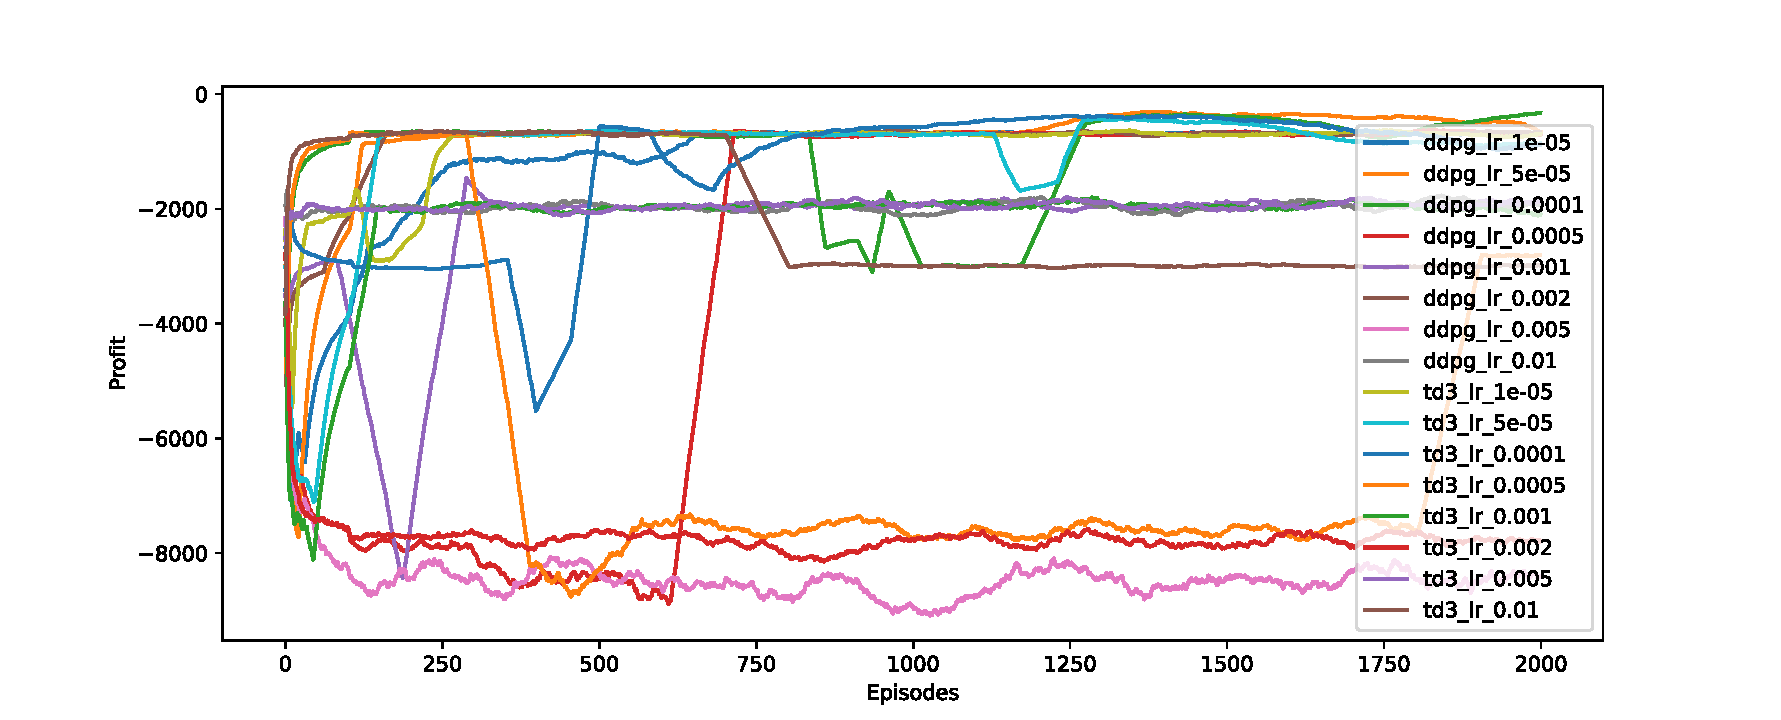
\includegraphics[width=\textwidth]{main/DDPG_learning_curve.pdf}
	\caption{Lernkurven von DDPG und TD3 mit unterschiedlichen Lernraten}
	\label{grafic:DDPGLearningCurve}
\end{figure}

Die Lernkurven der beiden sehr ähnlichen Verfahren DDPG und TD3 sind in Abbildung \ref{grafic:DDPGLearningCurve} dargestellt.
Für jeden der beiden Algorithmen wurden acht Trainingsläufe durchgeführt, die mit unterschiedlichen Lernraten parametrisiert wurden.
Der Standardwert liegt für beide Algorithmen bei $1e-3$.
Es wurden Trainingsläufe mit diesen Lernraten sowie kleineren und größeren durchgeführt.
Die beim Training beobachteten Muster gleichen sich sowohl bei den beiden Algorithmen als auch den unterschiedlichen Parametrisierungen.

Zu Beginn des Trainings ist bei einigen Läufen eine Verbesserung der gemittelten Returns, die primäre Leistungskennziffer, zu beobachten.
Allerdings kommt diese Verbesserung bei allen Algorithmen zum Erliegen und eine konstante Leistung stellt sich ein.
Dabei treten Häufungen bei der Leistung -2000 und -700 auf.
Bei einigen Trainingsdurchläufen wird ein Niveau von -300 erreicht, dieses aber nie überschritten.

\section{Trainingsdauer und Sample Efficiency}

\section{Stabilität}

\section{Analyse und Vergleich der ermittelten Policies}
